\documentclass[11pt]{article}
\usepackage{fullpage}
\usepackage{graphics,epsfig,color}
\usepackage[utf8]{inputenc,xcolor}
\usepackage{wrapfig}

\usepackage{times}
\usepackage{setspace}
\usepackage{amsmath,amsthm,amssymb}
%\usepackage[ruled,vlined,linesnumbered]{algorithm2e}
\usepackage{qtree}
\usepackage{subfigure}
\usepackage{url}



%for code from latexdraw
%\usepackage[usenames,dvipsnames]{pstricks}
%\usepackage{epsfig}
%\usepackage{pst-grad} % For gradients
%\usepackage{pst-plot} % For axes


\newtheorem{theorem}{Theorem}[section]
%\newtheorem{proposition}{Proposition}[theorem]
\newtheorem{corollary}{Corollary}[section]
\newtheorem{lemma}{Lemma}[section]
%\newtheorem{claim}{Claim}[section]
\newtheorem{problem}{Problem}
%\newtheorem{conjecture}{Conjecture}[section]
\newtheorem{definition}{Definition}[section]
\newtheorem{observation}{Observation}[section]
\newtheorem{example}{Example}[section]
\newtheorem{openproblem}{Open Problem}[section]
\newtheorem{fact}{Fact}[section]
%\newcommand{\qedsymb}{\hfill{\rule{2mm}{2mm}}}

\newcommand{\qedsymb}{\hfill{\rule{2mm}{2mm}}}
\newenvironment{proofsketch}{\begin{trivlist}
\item[\hspace{\labelsep}{\noindent Proof Sketch: }]
}{\qedsymb\end{trivlist}}



%the following few lines until usepackage{algorithm2e} is to avoid the
%conflicts of algorithm2e with other packages.
\makeatletter
\newif\if@restonecol
\makeatother
\let\algorithm\relax
\let\endalgorithm\relax
%\usepackage[ruled,vlined,linesnumbered]{algorithm2e}
\usepackage[ruled,vlined,linesnumbered]{algorithm2e}


%\newenvironment{proof}{\begin{trivlist}
%\item[\hspace{\labelsep}{\bf\noindent Proof: }]}{\qedsymb\end{trivlist}}
%\newcommand{\qed}{\hfill\rule{2mm}{2mm}}

\newcommand{\remove}[1]{}

\definecolor{myPurple}{HTML}{9E449E}
\definecolor{myBlue}{HTML}{44859E}
\definecolor{myGreen}{HTML}{5EC766}



%--------------------------------


\begin{document}

\begin{center}
  {\LARGE CSCD501 Homework1}

\bigskip 

{\Large Will Czifro}

\end{center}

\bigskip

\noindent{\bf Solution for Problem 1.}

This claim is false. Consider Figure 1. In this graph, the value in each node represents its degree. If we apply this approximation to this graph, the best case is that it consistantly selects all nodes in top row, which is the min cover for this graph. However, under the worst case all of the nodes of the bottom row are selected as the approximation. In this case, we have a ratio greater than 2. If $C*$ represents our min cover, then $|C*| = 10$ which we can achieve under best case scenario. For the worst case, $|C| = 27$. We then get a ratio $\frac{|C|}{|C*|} = $$\frac{27}{10} > 2$. This proves the claim to be false.

%---------------------------------------
\bigskip

\noindent{\bf Solution for Problem 2.}

For this problem, consider the example from Figure 2. We want to know if a peak is in line of view, or is it observable. We can determine if a peak effects the observability by comparing viewing angles. For example peaks beyond $h_3$ are not observable because their respective viewing angles are less than that of $h_3$. So to determin of a peak is observable, we must check if a peak prior to it has a greater viewing angle. To avoid taking a performance hit on calculating the viewing angle, we simply use the ratio that determines the angle, $\frac{h_i - h_0}{d_i}$ denoted as $r_i$ for all $i \in \{0,1,2,...,n-1\}$ where $n$ is the number of peaks.

Parallel prefix is the best method to solve this problem. Let the prefix $P$ have the following tuple structure: $P =
(r_j,r_m)$ where $r_j$ is a peak with a ratio greater than $r_i$, where $j \leq i$, and $r_m$ is the globally observed max ratio for the entire data set and $m$ is the position the ratio came from. When we exchange messages between processors, we only send $P.r_m$. When a processor receives a ratio, $r^{\prime}_j$, if $j \leq i$ and $P.r_j < r^{\prime}_j$ then $P.r_j$ gets updated to that value. Likewise, $P.r_m$ gets updated if $r^{\prime}_j > P.r_m$. When communication stops, all processors will have the same $r_m$ and each processor will have a there own $r_j$. The $ith$ peak can be determined to be observable if $r_i \geq P.r_j$ and $i < m$. Otherwise, $peak_i$ is not observable. Consider Algorithm 1.


\newpage

\begin{figure}[h!]
\begin{center}
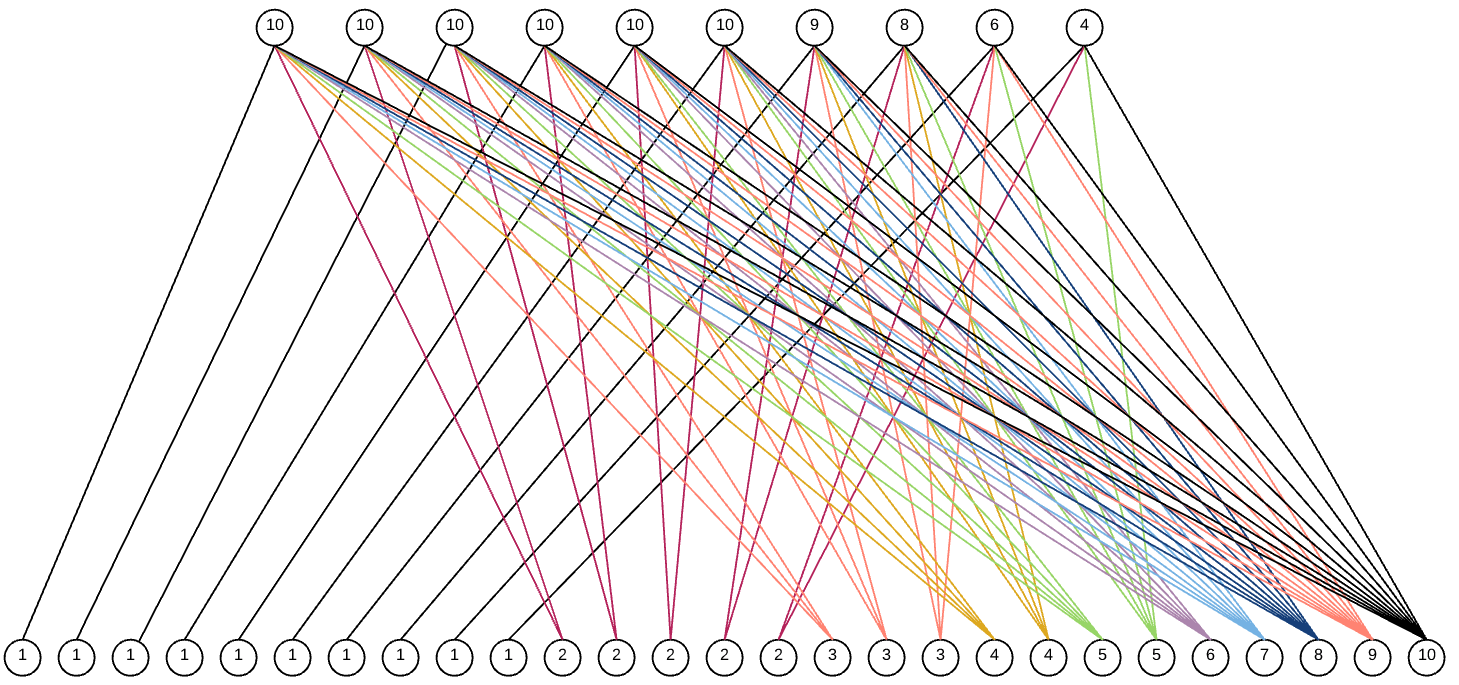
\includegraphics[scale=0.3]{Figure1.png}
\caption{Bipartite Graph}
\label{fig:bipart}
\end{center}
\end{figure}

\begin{figure}[h!]
\begin{center}
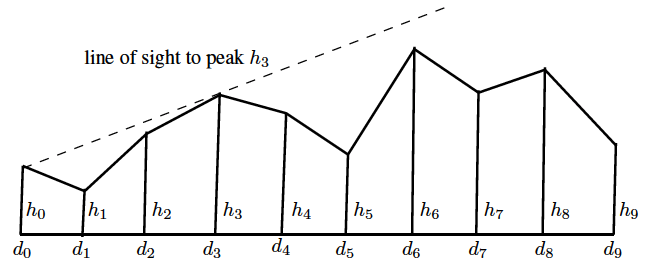
\includegraphics[scale=0.4]{Figure2.png}
\caption{Graph of Mountain Peaks}
\label{fig:peaks}
\end{center}
\end{figure}

\newpage

\begin{algorithm}
\DontPrintSemicolon
\SetKwInOut{Input}{input}\SetKwInOut{Output}{output}
\SetKw{KwTo}{t}
\Input{heights is an array of all peak heights\\
       distances is an array of horizontal peak distances\\
       startHeight is the height of the observer}
\Output{a boolean array representing the observability for each peak}
\BlankLine
Processors have ids $0,1,..,n-1$, represented by a d-bit string, where $d = log_2 p$\;
Assign each processor a peak ratio\;
Let o be the boolean array representing the observability for each peak\;

\tcc{Code on one processor}
Let P be the local prefix\;
Initial $P.r_j$ and $P.r_m$ to be $r_i$ and set $o_i$ to true\;

\For{$k = 0$ to $d-1$}{
  1) Exchange $P.r_m$ with the processor whose id is obtained by flipping the ith bit\;
  2) If received $r^{\prime}_j$ is from smaller pid and $r^{\prime}_j > P.r_j$ update $P.r_j$ with $r^{\prime}_j$\;
  3) If $r^{\prime}_j \geq P.r_m$ then update $P.r_m$\;
}

If $P.r_j > r_i$ or ($P.r_m > r_i$ and $m < i$) then set $o_i$ to false\;

\tcc{End code on one processor}

\Return{o}
\caption{PeakObservability\_Parallel(heights,distances,startHeight)}\label{algo_Y}
\end{algorithm}

\end{document}

